\documentclass[11pt]{beamer}


\usepackage{amssymb, amsmath, graphicx, caption, enumerate}
\graphicspath{ {images/} }
\usepackage{amsthm}
\usepackage{xargs}
\usepackage{scalerel}




\newcommand{\N}{\mathbb{N}}
\newcommand{\Z}{\mathbb{Z}}
\newcommand{\R}{\mathbb{R}}
\newcommand{\K}{\mathbb{K}}
\newcommand{\C}{\mathbb{C}}
\newcommand{\D}{\mathcal{D}}
\newcommand{\A}{\mathcal{A}}
\newcommand{\ds}{\displaystyle}
\newcommand{\op}[1]{\left(#1\right)}
\newcommand{\cp}[1]{\left[#1\right]}
\newcommand{\av}[1]{\left| #1\right|}
\newcommand{\st}[1]{\left\{#1\right\}}


\usepackage[colorinlistoftodos,prependcaption,textsize=tiny]{todonotes}
\newcommandx{\question}[2][1=]{\todo[linecolor=red,backgroundcolor=red!25,bordercolor=red,#1]{#2}}
\newcommandx{\change}[2][1=]{\todo[linecolor=blue,backgroundcolor=blue!25,bordercolor=blue,#1]{#2}}
\newcommandx{\add}[2][1=]{\todo[linecolor=OliveGreen,backgroundcolor=OliveGreen!25,bordercolor=OliveGreen,#1]{#2}}
\newcommandx{\improve}[2][1=]{\todo[linecolor=Plum,backgroundcolor=Plum!25,bordercolor=Plum,#1]{#2}}
\newcommandx{\thiswillnotshow}[2][1=]{\todo[disable,#1]{#2}}
\newcommandx{\remove}[2][1=]{\todo[linecolor=yelllow,backgroundcolor=yellow!10,bordercolor=red,#1]{#2}}


\newcommand\reallywidehat[1]{\arraycolsep=0pt\relax%
\begin{array}{c}
\stretchto{
  \scaleto{
    \scalerel*[\widthof{\ensuremath{#1}}]{\kern-.5pt\bigwedge\kern-.5pt}
    {\rule[-\textheight/2]{1ex}{\textheight}} %WIDTH-LIMITED BIG WEDGE
  }{\textheight} % 
}{0.5ex}\\           % THIS SQUEEZES THE WEDGE TO 0.5ex HEIGHT
#1\\                 % THIS STACKS THE WEDGE ATOP THE ARGUMENT
\rule{-1ex}{0ex}
\end{array}
}


\usetheme{CUDenver}
\renewcommand{\familydefault}{\sfdefault}
\usefonttheme[onlymath]{serif}
\usepackage{tikz}
\usetikzlibrary{arrows}
\setbeamertemplate{itemize items}{>>}
\setbeamertemplate{itemize subitem}[square]
\setbeamertemplate{itemize subsubitem}[ball]
\newcommand{\norm}[1]{\left\lVert#1\right\rVert}



\author{Jordan R. Hall}

\title[CUDenver Theme]{Thesis Proposal}

\institute[UCD]{
Department of Mathematical and Statistical Sciences\\
University of Colorado Denver
}

\date{Tuesday, December 4, 2018}

\begin{document}
% ------------------------------------------------


\begin{frame}[t,plain]
    \titlepage
\end{frame}

% start the content of the presentation

\begin{frame}{Overview}
\tableofcontents
\end{frame}


% ------------------------------------------------
\section{Literature Review and Framework}
% ------------------------------------------------
\begin{frame}

\begin{center}
\textbf{Notation}
\end{center}

\begin{itemize}

	\item We define a parameter space $\Lambda$ with dimension $N$ and a data space $\mathcal{D}$ with dimension $M$. Generally $M \leq N$.
	
	\item We define a parameter-to-data map $f$, which is noisy and $\nabla f$ may be inaccessible.
	
	
	\item We write $d=f(\lambda) \in \mathcal{D}$ to denote a particular datum corresponding to the evaluation of a point $\lambda \in \Lambda$.

\end{itemize}

\end{frame}

% ------------------------------------------------
\subsection{Data-Consistent Inversion (DCI)}
% ------------------------------------------------

\begin{frame}

\begin{itemize}

	\item Following Butler, Stuart, and Tarantola, we formulate the Stochastic Inverse Problem (SIP).
	
	\item  We define prior knowledge of the parameter space, given by the \emph{prior distribution}, $\pi_\Lambda^\text{prior}(\lambda)$.

	\item We define the \emph{observed distribution}, $\pi_\mathcal{D}(d)$, which represents our uncertain state of knowledge of observed data.
	
	\item The SIP is the task of finding an \emph{updated} probability distribution, $\pi_\Lambda^\text{update}$, in $\Lambda$ space that combines the given prior information and data.
	

\end{itemize}



\end{frame}


\begin{frame}

\begin{itemize}

\item Given a distribution on $\lambda \in \Lambda$, the \emph{forward Uncertainty Quantification (UQ) problem} is finding the probability distribution of $f(\lambda)$. The forward UQ problem is, in its own right, a nontrivial and important problem in UQ.

\item The \textit{classical Bayesian} or \textit{statistical Bayesian} solution to the inverse problem is not generally a 
\textit{pull-back probability measure}, meaning the image of the updated distribution $\pi_\Lambda^\text{update}$ under the map $f$, called the \textit{push-forward} of $\pi_\Lambda^\text{update}$, is not equal to the observed probability distribution, $\pi_\mathcal{D}$. 


\end{itemize}

\end{frame}

\begin{frame}

\begin{itemize}

	\item Data-consistent inversion (DCI) seeks an updated solution $\pi_\Lambda^\text{update}$ for which the push-forward exactly equals $\pi_\mathcal{D}$. 
	
	\item To obtain such a solution, we must solve the forward problem $f(\pi_\Lambda^\text{prior})$.
	
	\item We denote the solution to the forward problem with $\pi_\mathcal{D}^{f(\Lambda)}(d)$.




	\item As in Butler, the data-consistent solution to the SIP is 
	
\begin{equation} \label{eq:1}
\pi_\Lambda^\text{update}(\lambda)=\pi_\Lambda^\text{prior}(\lambda)\frac{\pi_\mathcal{D}(f(\lambda))}{\pi_\mathcal{D}^{f(\Lambda)}(f(\lambda))}.
\end{equation}

	
\end{itemize}


\end{frame}

% ------------------------------------------------
\subsection{Optimization Methods for Solving Inverse Problems}
% ------------------------------------------------

\begin{frame}

\begin{itemize}

	\item With an expensive $f$ and large $N$, approximately solving the forward UQ problem needed to form \eqref{eq:1} generally requires density estimation which converges at best near a Monte Carlo $\mathcal{O}\left(\frac{1}{\sqrt{N}} \right)$ convergence rate.
	
	\item In the case that $f$ is a linear operator and the prior and observed densities are Gaussians, the solution to the SIP can be obtained exactly, and its mean is equivalent to the solution of a deterministic convex optimization problem.
	
	\begin{itemize}
		\item The classical formulation of the objective function (Tarantola) can be altered (Wildey, Butler, et al) to obtain a data-consistent (approximate) solution with $f$ linear and Gaussian $\pi_\Lambda^{\text{prior}},$ $\pi_\mathcal{D}$.
	\end{itemize}

\end{itemize}

\end{frame}


\begin{frame}

\begin{itemize}
	
	\item With $f$ linear, we define its matrix $A$. Given observed data $d_{\text{obs}} \sim \pi_\mathcal{D}$ and a draw $\lambda_\text{prior}\sim \pi_\Lambda^\text{prior}$, as in Tarantola, we define the \textit{classical misfit function,}


\begin{equation} \label{eq:2}
S(\lambda)=\frac{1}{2}\left(\left|\left|C_\mathcal{D}^{-1/2}(A\lambda-d_{\text{obs}})\right|\right|_2^2+\left|\left|C_\Lambda^{-1/2}(\lambda-\lambda_{\text{prior}})\right|\right|_2^2\right).
\end{equation} 

\item In Tarantola, it is assumed that $\pi_\Lambda^\text{prior}$ and $\pi_\mathcal{D}$ are Gaussians, and the misfit function is specified by $\lambda_{\text{prior}}=\bar{\lambda}$ and $d_{\text{obs}}=\bar{d}$, the respective means of the prior and observed densities.

\item The minimum of $S$ is called the maximum a posteriori point, or \textit{MAP point}, $\lambda_S^*$, and the classical solution to the SIP is $\pi_\Lambda^\text{update}(\lambda) = c\cdot \exp(-S(\lambda)),$ where $c$ is a constant.


\end{itemize}


\end{frame}



\begin{frame}

\begin{itemize}




	\item Widley, Butler, et al reformulate $S$ to write an objective function with a minimizer which is a data-consistent MAP point. 
	
		\item An additional ``deregularization" term is appended so that if a unique solution exists, the regularization will be ``turned off." We write the \textit{data-consistent misfit function,}
	
	
	
$$T(\lambda)=\frac{1}{2}\left(\left|\left|C_\mathcal{D}^{-1/2}(A\lambda-d_{\text{obs}})\right|\right|_2^2+\left|\left|C_\Lambda^{-1/2}(\lambda-\lambda_{\text{prior}})\right|\right|_2^2\right)$$
	

\begin{equation} \label{eq:3}
-\frac{1}{2}\left(\left|\left|C_A^{-1/2}(A\lambda-A\lambda_{\text{prior}})\right|\right|_2^2\right),
\end{equation} 

\noindent where $C_A=AC_\Lambda A^T$. 
	



\end{itemize}

\end{frame}


\begin{frame}



\begin{itemize}

	\item We call the minimum of $T$, $\lambda_T^*$, the data-consistent MAP point.

	\item In the case that $\pi_\Lambda$ and $\pi_\mathcal{D}$ are Gaussian, the data-consistent solution to our inverse problem is given exactly by $\pi_\Lambda^\text{update}(\lambda_T^*)= c\cdot \exp(-T(\lambda))$. 

	\item The deregularization term will ensure a solution that updates the distribution on $\Lambda$ in the directions in which the data is informative. 



\end{itemize}



\end{frame}


\begin{frame}

\noindent \textbf{Example 1.} Let $f(\lambda)=2\lambda$, $\lambda_\text{prior}=0.1$, $C_\Lambda=[0.5],$ $d_\text{obs}=0.25$, and $C_\mathcal{D}=[0.25]$; note, $N=M=1$. Then we find that 

$$S(\lambda)=2((2\lambda-0.25)^2+(\lambda-0.1)^2),$$ 

\noindent which is minimized by $\lambda^*_S=3/25$. Assuming that $\lambda_\text{prior}$ and $d_\text{obs}$ are the means of Gaussians with variances corresponding to the above covariance matrices, we have $\pi_\Lambda^\text{post} \sim \exp(-S(\lambda))$ with mean $\lambda_S^*$. Notice $f(\lambda^*_S)=6/25\neq d_\text{obs}$. We write 
$$T(\lambda)=2(2\lambda-0.25)^2,$$ 

\noindent which is minimized by $\lambda^*_T=1/8$. Notice $f(\lambda^*_T)=d_\text{obs}$. With Gaussian assumptions on the prior and data, we have $\pi_\Lambda^\text{post} \sim \exp(-T(\lambda))$ with mean $\lambda_T^*$.



\end{frame}


\begin{frame}

\noindent \textbf{Example 2.} Let $f(\lambda)=2\lambda_1-\lambda_2$, $\lambda_\text{prior}=(0.1 \quad 0.2)^\top$, $C_\Lambda=\text{diag}[0.5,0.25],$ $d_\text{obs}=0.1$, and $C_\mathcal{D}=[0.25]$.

\vspace{0.25cm}

 With $N=2$ and $M=1$, for any $\lambda \in \Lambda$, $f(\lambda)=d=2\lambda_1-\lambda_2$. Since there is just a single $d_\text{obs}$, we have $0.1=2\lambda_1-\lambda_2$.

\vspace{.25cm}

We find $S$ is minimized by $\lambda^*_S=(7/50,19/100)$. 
Assuming that $\lambda_\text{prior}$ and $d_\text{obs}$ are the means of Gaussians with variances corresponding to the given covariance matrices, we have $\pi_\Lambda^\text{post} \sim \exp(-S(\lambda_S))$ with mean $\lambda_S^*$. Notice $f(\lambda^*_S)=9/100\neq d_\text{obs}$. 

\vspace{.25cm}
 
In the data-consistent formulation, we have 
$T$ minimized by $\lambda^*_T=(13/90,17/90)$. Notice $f(\lambda^*_T)=9/90=d_\text{obs}$. With Gaussian assumptions, we have $\pi_\Lambda^\text{post} \sim \exp(-T(\lambda))$ with mean $\lambda_T^*$. 



\end{frame}

\begin{frame}


\begin{figure} 
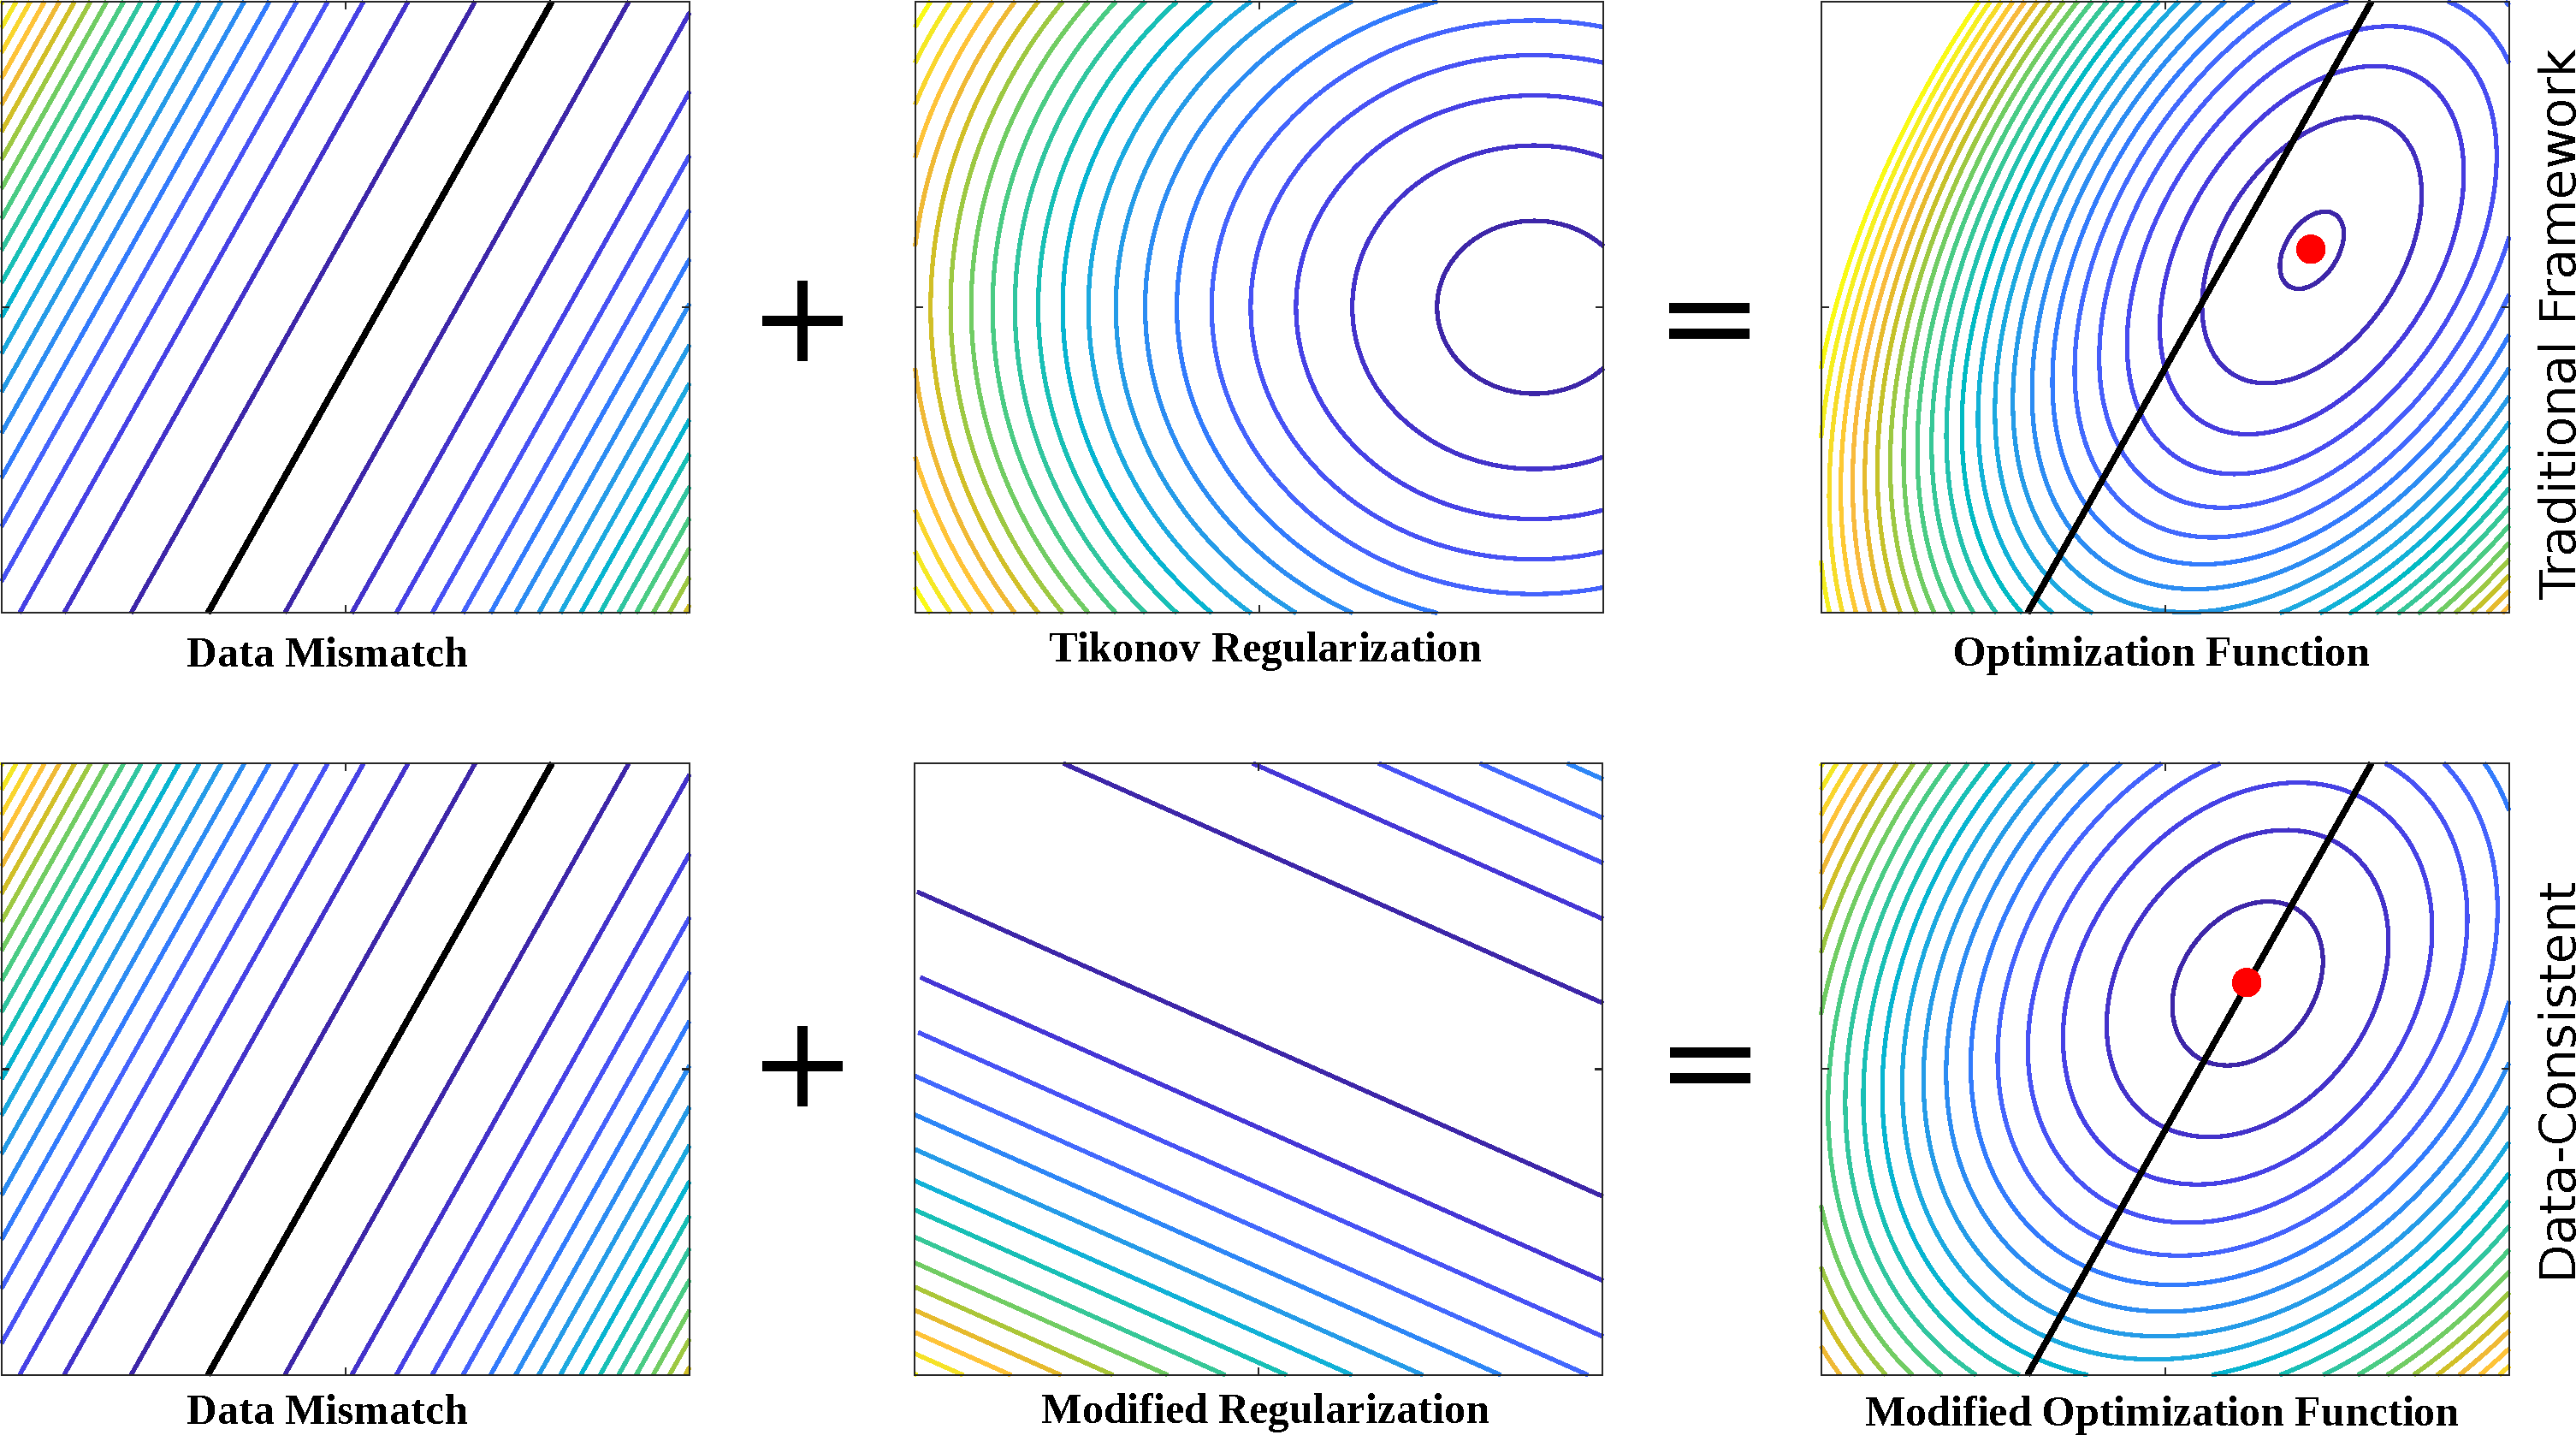
\includegraphics[scale=0.2]{Regularization-all-in-one.pdf}

This figure from Wildey, Butler, et al shows the process of obtaining the statistical/classical Bayesian solution and data-consistent solution in Example 2.
\end{figure}

\end{frame}

% ------------------------------------------------
\subsection{Dimension Reduction}
% ------------------------------------------------

\begin{frame}

\begin{itemize}

	\item We consider functions $f: \Lambda \to \mathcal{D}$ where $\dim(\Lambda)=N$ is large and $\dim(\mathcal{D})=M$ is such that $M<N$ or $M<<N$.

\begin{itemize}
		\item Functions of interest may represent postprocessed quantities from the solution of complex physical models.
\end{itemize}

\item It is not often that every parameter has equal impact on function values -- usually some parameters matter more than others.

\item The dimension reduction techniques considered seek to explain outputs $f(\Lambda)$ in an \textit{active subspace} $\mathcal{A} \subset \Lambda$ for which $\dim(\A)<N.$

\begin{itemize}
\item A lower-dimensional representation of $f$ can save computational costs.

\end{itemize}


\end{itemize}


\end{frame}

\begin{frame}

\begin{itemize}

\item $\nabla f(\lambda)\in \Lambda$ is a column vector with rows containing the $N$ partial derivatives of $f$, which for this discussion we assume exist, and are square integrable in $\Lambda$ equipped with some probability density that is positive everywhere in $\Lambda$ and 0 otherwise.

\begin{itemize}
		\item We consider $\pi_\Lambda^\text{prior}(\lambda)$, the density describing our prior state of knowledge, which we abbreviate as $\pi_\Lambda$.
\end{itemize}

\item One transforms inputs $\lambda$ to the origin with some fixed variance, typically so that $\lambda\in [-1,1]^N$. Then, as in Const. MC, we define

\begin{equation} \label{eq:4}
W=\int_\Lambda \nabla f(\lambda) \nabla f(\lambda)^\top  \pi_\Lambda(\lambda) d\lambda,
\end{equation} 

\noindent which is an $N\times N$ symmetric positive semi-definite matrix.

\end{itemize}

\end{frame}

\begin{frame}

\begin{itemize}



\item Interpreting $W$ as a certain covariance structure over $\Lambda$ leads one to the idea of computing the Singular Value Decomposition of $W$,

\begin{equation} \label{eq:5}
W=U\Sigma V^*,
\end{equation} 

\noindent where $U$ is $N \times N$ unitary, $\Sigma$ is $N \times N$ diagonal with the singular values of $W$ along its diagonal, and $V^*$ is $N \times N$ unitary.

\item We plot the singular values, $\{\sigma_i\}_{i=1}^n$ and seek a drop-off in magnitude between some pair of singular values, $\sigma_{j}$ and $\sigma_{j+1}$. The active subspace is the span of $u_1,\ldots,u_{j}$, which are the first $j$ columns of $U$, the left singular vectors of $W$. 


\end{itemize}

\end{frame}

\begin{frame}

\begin{itemize}

	\item For a point $\lambda \in \Lambda$, we define

\begin{equation} \label{eq:6}
  \mathcal{P}_\A(\lambda)=\sum_{i=1}^{j}\left( u_i^T \lambda\right)u_i \in \A, 
\end{equation}

\noindent which is the projection of $\lambda$ in the active directions of $f$. We call this projection an active variable, which is a point in the active subspace $\A$. 

\item We have arrived at the property that 

\begin{equation} \label{eq:7}
f\left(\mathcal{P}_\A(\lambda)\right) \approx f(\lambda).
\end{equation}


\end{itemize}



\end{frame}


\begin{frame}

\begin{itemize}

\item In practice, finding an active subspace of $f$ requires forming an approximation to $W$ via Monte Carlo. Here we consider a method by Russi.



\item We define $D_S=\{(\lambda_i,f(\lambda_i))\}_{i=1}^S$, a set of $S$ pairs of samples $\lambda_i \in \Lambda$ and their function values. One may use $D_S$ to approximate $\nabla f$. We denote each estimation to $\nabla f(\lambda_i)$ with $\reallywidehat{\nabla f}(\lambda_i)$.

\item We form the $N \times S$ matrix $\tilde{W}$ (which we present as $\tilde{W}^\top$)

\begin{equation} \label{eq:9}
\tilde{W}^\top:=\begin{bmatrix}
\reallywidehat{\nabla f}(\lambda_1)
\cdot \cdot \cdot
\reallywidehat{\nabla f}(\lambda_S)\\
\end{bmatrix}.
\end{equation}  


\end{itemize}


\end{frame}

\begin{frame}

\begin{itemize}

	\item Forming the SVD of $\tilde{W}$, $\tilde{W}=\tilde{U}\tilde{\Sigma}\tilde{V}^*$, we search for a drop off in the magnitude of the singular values $\{\tilde{\sigma}_i\}_{i=1}^S$. Assuming such a drop off occurs for an index $j:1<j<S$, we have the $j$ corresponding left singular vectors,$ \tilde{u},\ldots,\tilde{u}_{j}$.  
	
	\item Then $$\A\left(f; D_S \right):=\text{span}\{\tilde{u},\ldots,\tilde{u}_{j}\}$$ is the active subspace of $f$ with respect to the samples $D_S$.

	\item We check the extent to which the active subspace accounts for functions values $f(\lambda)$ 
by checking for resolution in a \emph{sufficient summary plot}, where we plot active variables against function values.


\end{itemize}



\end{frame}

% ------------------------------------------------
\subsection{Derivative-Free Optimization (DFO)}
% ------------------------------------------------

\begin{frame}

\begin{itemize}

\item Many important physical systems possess turbulent or chaotic behavior.  The physical state of the system $u(x,\lambda)$ and the corresponding parameter
to observable map $f(u(x,\lambda))$ may be modeled as a stochastic process, or as a deterministic function with additive or multiplicative noise.  

\begin{itemize}


\item In this setting, the efficient extraction of accurate gradients of $f$ in parameter space is a challenging undertaking, as popular techniques based on
linearization, including adjoint methods, are inaccurate (Lea/Qiqi).  

\item The finite-difference approximations to $\nabla f_\Lambda$ 
involve $N=\text{dim}\Lambda$ 
additional, usually nonlinear model solves for the physical system state $u(x,\lambda_i + \delta \lambda_i)$, and is greatly polluted by the noise in $f$.

\end{itemize}


\end{itemize}


\end{frame}

\begin{frame}

\begin{itemize}
 


\item We consider derivative-free optimization (DFO) algorithms suited for additive and multiplicative noise (). This technique requires nothing more than evaluations of the noisy model and random draws from a normal distribution.


\begin{itemize}


\item The method finds a new iterate by randomly perturbing the previous iterate in $\Lambda$.

\item Iterates are not allowed to stray much due to relatively small smoothing factors and step sizes. The smoothing factor and step size in the DF algorithms are of great importance to their convergence and termination. 

\item The smoothing factor and step size will depend on a scale factor of the $L_1$ Lipschitz constant of $f$. It is of interest to obtain estimates of $L_1$, which is not straightforward in a gradient-free setting. We refer to 2 papers () for Lipschitz constant learning.


\end{itemize}

\end{itemize}

\end{frame}


\begin{frame}

\begin{itemize}
	
	\item We consider the problem

\begin{eqnarray} \label{eq:9}
\min_{\lambda \in \R^N} \quad \mathbb{E}\left[f(\lambda)+\nu (\lambda; \epsilon)\right],
\end{eqnarray} 

\noindent where:

\begin{enumerate}[(i.)]

\item $f: \R^N \to \R$ is convex;

\item $\epsilon$ is a random variable with probability density $P(\epsilon)$;

\item for all $\lambda$ the additive noise model $\nu$ is independent and identically distributed, has bounded variance $\sigma_a^2$, and is unbiased; i.e., $\mathbb{E}_\epsilon (\nu(\lambda;\epsilon))=0$.

\end{enumerate}

\end{itemize}

\end{frame}


\begin{frame}

\begin{itemize}

	\item We consider algorithms such as \textit{STARS (STep-size Approximation in Randomized Search)}, which: 

\begin{itemize}
		\item uses small perturbations in the domain $\Lambda=\R^N$ by the addition of a random vector with components drawn from a normal distribution to iterates $\lambda^{(k)}$; 
		\item computes the function value at the randomly perturbed point with additive or multiplicative noise drawn from a specified distribution; 
		\item and updates iterates using a Gaussian-smoothed finite-difference scheme for approximate gradient information in a gradient descent fashion. 

\end{itemize}

\end{itemize}



\end{frame}




% ------------------------------------------------
\section{Research Questions}
% ------------------------------------------------


% ------------------------------------------------
\subsection{Data-Consistent Deregularization for Nonlinear $f$}
% ------------------------------------------------

\begin{frame}

\begin{itemize}
	
	\item For a general nonlinear map $f$, we must reformulate the deregularization which we recall for a linear map $f$ with matrix $A$ may be written

\begin{equation} \label{eq:10}
\left|\left|C_A^{-1/2}(A\lambda-A\lambda_{\text{prior}})\right|\right|_2^2,
\end{equation} 

\noindent where $C_A=AC_\Lambda A^\top$. 

\item For a nonlinear $f$, we may expand $f$ linearly around some $\lambda \in \Lambda$ and write $f(\lambda)-f(\lambda_\text{prior})=A (\lambda-\lambda_\text{prior})$, where $A=\nabla f (\lambda)^\top$, which is an $N \times M$ matrix. In order to fully determine the form of \eqref{eq:10}, we must find $(f(\lambda)^\top C_\Lambda f(\lambda))^{-1}$.


\end{itemize}

\end{frame}

% ------------------------------------------------
\subsection{Impact of Noise on MAP Point and Updated Prior}
% ------------------------------------------------

\begin{frame}

\begin{itemize}

	\item The effects of noise on individual methods considered in this paper -- particularly: DCI, the deterministic optimization solution for SIPs, active subspaces, and DFO -- have been characterized to varying extents in corresponding literature. 
	
\begin{itemize}

		\item 	We investigate the impact of additive and multiplicative noise models in our framework, which may involve embedding the aforementioned methods in one another, performing them in series, or both.

\end{itemize}	


\item Formally, we investigate both sensitivity and stability of any proposed methods. 

\begin{itemize}

		\item Theoretically, this may involve using the individual sensitivity/stability analyses of certain methods while deriving new results when the methods are embedded or performed in series. 
		

\end{itemize}


\end{itemize}

\end{frame}

% ------------------------------------------------
\subsection{Learning and Sampling}
% ------------------------------------------------

\begin{frame}

\begin{itemize}

	\item We are interested in several problems that involve sampling $\Lambda$ and evaluating $f$ including solving the forward problem, finding an active subspace via Monte Carlo, and performing DFO.
	
	\begin{itemize}
	
		\item We are interested in comparing active subspaces obtained from sampling $f$ with few samples, or with samples generated from some other process, such as a DFO algorithm.
		
		\item 	Since many DFO algorithms use hyperparameters for step sizes and smoothing that depend on $L_1$, the literature () contains attempts to learn Lipschitz constants from sampling alone.
	
	\end{itemize}


\end{itemize}

\end{frame}


% ------------------------------------------------
\subsection{Using the Active Subspace}
% ------------------------------------------------

\begin{frame}

\begin{itemize}

	\item Computational expense may be saved by projecting points $\lambda$ into their active variables, since such projections are of lower dimension than $\Lambda$. 
	
	\item This property gives the ability to save computational expense for a number of problems in Uncertainty Quantification, including optimization, representation and solving inverse problems.

\end{itemize}

\end{frame}




% ------------------------------------------------

\section{Preliminary Results and Research Plan}
% ------------------------------------------------
\begin{frame}

$x$

\end{frame}




% ------------------------------------------------
\section{Timeline}
% ------------------------------------------------
\begin{frame}

We outline a rough timeline for the remaining 2 years in a 5.5 year plan.

\begin{itemize}
\tiny

\item Clean existing algorithms and examples, generate richer research results related to DFO and active subspaces, and build a model inverse problem for investigation. (Dec 2018/Jan 2019)

\item On RA for Spring 2019.

\item Write and present MS-level results. (Feb/Mar 2019)

\item Work on theoretical formulation of deregularization for nonlinear $f$. Work on generating notebooks and examples. (Ongoing/Spring and Summer 2019)

\item Summer research; begin writing thesis; summer school/internship/conference (?) (Jun/Jul/Aug 2019)

\item Fall 2019 - Writing phase, revisions.

\item Spring 2020 - Final revisions, software.

\item Summer 2020 Internship/collaborations, publishing, formatting.

\item Defend thesis Summer 2020 or early Fall 2020.


\end{itemize}


\end{frame}



% ------------------------------------------------

\section{References}
% ------------------------------------------------
\begin{frame}

$x$

\end{frame}







\end{document}

